\documentclass{article}
\usepackage[utf8]{inputenc}
\usepackage{CJKutf8}  %输入中文
\usepackage{amsmath}  %数学公式
\usepackage{amssymb} 
\usepackage{setspace} %使用间距宏包
\usepackage{geometry} %设置页面边距、页面大小的宏包
\usepackage{graphicx} %插入图片的宏包

\usepackage{hyperref} %链接宏包
\hypersetup{
    colorlinks=true,
    linkcolor=blue,
    filecolor=magenta,      
    urlcolor=cyan,
}

%\geometry{a4paper,scale=0.8} %版心占页面比例为80%
\geometry{a4paper,left=2.5cm,right=2.5cm,top=1cm,bottom=2cm}

\newcommand{\subf}[2]{	% 设置多图排版
  {\small\begin{tabular}[t]{@{}c@{}}
  #1\\#2
  \end{tabular}}%
}

\title{
	\begin{LARGE}
		\textbf{Solutions to Assignment 2}
	\end{LARGE}
	}	

\author{18214613 陈承勃}

\date{Dec 31st, 2018}

\begin{document}
\begin{CJK}{UTF8}{gbsn}
\maketitle
\end{CJK}
\begin{spacing}{1.5} %设置行间距

\section*{Abstract}
In this report, I first derive the mathematical solutions for Gaussian Mixtures using EM algorithm from scratch in \textbf{Section 1}, and give a general framework of EM algorithm for GMM. In \textbf{Section 2}, I display my solutions to \textbf{Assignment 2} based on the theoretical results I derived. The results of my experiments show that EM algorithm can be well applied to Gaussian mixtures, and is quite sensitive to the initialization of parameters, that is, under different initializations, not only the speed of convergence variates, but also the training get down to different convergence. The experiments are implemented using MATLAB.

\section{Framework of EM Algorithm for GMM model}
\subsection{Notations}
In this section, I will derive the mathematical solution for Gaussian Mixed Model using EM algorithm, that is, to give a general framework of how EM algorithm serves GMM model. 

Suppose we have observations $X = \{x^{(1)}, x^{(2)}, \dots, x^{(N)}\}$, where $x^{(n)}=(x^{(n)}_1, x^{(n)}_2, \dots, x^{(n)}_d)^T$. Then, the Gaussian mixture distribution for each observation $x^{(n)}$ can be written as
\begin{equation}
p(x^{(n)}) = \sum_{k=1}^{K}\pi_k \mathcal{N}(x^{(n)}|\mu_k, \Sigma_k)
\end{equation}

Let $Z=(z^{(1)}, z^{(2)}, \dots, z^{(N)})$. The corresponding latent variable $z^{(n)}$ is a K-dimensional binary random variable which satisfies $z^{(n)}_k\in\{0,1\}$ and $\sum_k z^{(n)}_k = 1$, where $K$ denotes the number of Gaussians. The corresponding mixing coefficients $\pi_k$ specifies the marginal distribution over $z^{(n)}$, such that
\begin{equation}
p(z^{(n)}_k=1)=\pi_k
\end{equation} 
where the parameters $\{\pi_k\}$ must satisfy 
\begin{equation}
0 \leq \pi_k \leq 1
\end{equation}
together with
\begin{equation}
\sum_{k=1}^K \pi_k = 1
\end{equation}
Because $z^{(n)}$ uses a $1$-of-$K$ representation, we can also write the distribution of $z^{(n)}$ as
\begin{equation}
p(z^{(n)}|\pi)= \prod_{k=1}^K \pi_k^{z^{(n)}_k}
\end{equation}

\subsection{Training Objective}
Therefore, the \textbf{in-complete likelihood} is given by 
\begin{equation}
p(X|\pi,\mu,\Sigma) = \prod_{n=1}^N \sum_{k=1}^K \pi_k \mathcal{N}(x^{(n)}|\mu_k, \Sigma_k)
\end{equation}
And the corresponding \textbf{in-complete log-likelihood} is
\begin{equation}
\ln p(X|\pi,\mu,\Sigma) = \sum_{n=1}^N \sum_{k=1}^K \pi_k \mathcal{N}(x^{(n)}|\mu_k, \Sigma_k)
\end{equation}

Note that a summation over $k$ is inside the logarithm term which makes it hard to derive the solution. Thus we choose to maximize the much more simple but identical \textbf{complete likelihood}
\begin{equation}
p(X,Z|\pi,\mu,\Sigma)=\prod_{n=1}^N \prod_{k=1}^K [\pi_k \mathcal{N}(x^{(n)}|\mu_k,\Sigma_k)]^{z^{(n)}_k}
\end{equation}
That is, to maximize the \textbf{complete log-likelihood}
\begin{equation}
\ln p(X,Z|\pi,\mu,\Sigma)=\sum_{n=1}^N \sum_{k=1}^K z^{(n)}_k [\ln \pi_k + \ln \mathcal{N}(x^{(n)}|\mu_k, \Sigma_k)]
\end{equation}

According to the analysis above, \textbf{the objective of the EM algorithm is to maximize the complete log-likelihood}.

\subsection{E-step}
Given $\pi^{old}, \mu^{old}, \Sigma^{old}$, \textbf{the objective of the E-step is to take expectation of the complete log-likehood with respect to the latent variables} $Z$, i.e.,
\begin{equation}
E_Z [\ln p(X,Z|\pi,\mu,\Sigma)|X,\pi^{old}, \mu^{old}, \Sigma^{old}] = \sum_{n=1}^N \sum_{k=1}^K E_Z[z^{(n)}_k|x^{(n)}, \pi^{old}, \mu^{old}, \Sigma^{old}][\ln \pi_k + \ln \mathcal{N}(x^{(n)}|\mu_k, \Sigma_k)]
\label{E-step}
\end{equation}
And we denote
\begin{equation}
\begin{aligned}
\gamma(z^{(n)}_k)\equiv E_Z[z^{(n)}_k|x^{(n)}, \pi^{old}, \mu^{old}, \Sigma^{old}] &= \sum_{z^{(n)}_k} p(z^{(n)}_k|x^{(n)}, \pi^{old}, \mu^{old}, \Sigma^{old}) \\
&=\sum_{z^{(n)}_k}z^{(n)}_k \frac{p(z^{(n)}_k, x^{(n)}| \pi^{old}, \mu^{old}, \Sigma^{old}}{\sum_{k=1}^K p(z^{(n)}_k|x^{(n)}, \pi^{old}, \mu^{old}, \Sigma^{old})} \\
&= \frac{\pi_k \mathcal{N}(x^{(n)}|\mu_k, \Sigma_k)}{\sum_{k=1}^K \mathcal{N}(x^{(n)}|\mu_k, \Sigma_k)}
\end{aligned}
\end{equation}

\subsection{M-step}
\textbf{The objective of the M-step is to search for new parameters $\pi, \mu, \Sigma$, which maximize Eqn.\ref{E-step}}, that is, 
\begin{equation}
\begin{aligned}
& \underset{\pi, \mu, \Sigma}{\text{max}} 
& &\sum_{n=1}^N \sum_{k=1}^K \gamma(z^{(n)}_k)[\ln \pi_k + \ln \mathcal{N}(x^{(n)}|\mu_k, \Sigma_k)] \\
& \textbf{s.t.} & & \sum_{k=1}^K \pi_k = 1
\end{aligned}
\label{M-step}
\end{equation}
The \textit{Lagrangian} function of the optimization problem \ref{M-step} is given by
\begin{equation}
\mathcal{L} = \sum_{n=1}^N \sum_{k=1}^K \gamma(z^{(n)}_k)[\ln \pi_k + \ln \mathcal{N}(x^{(n)}|\mu_k, \Sigma_k)] + \lambda (\sum_{k=1}^K \pi_k - 1)
\end{equation}
where $\lambda > 0$
\subsubsection{Solution for $\pi$}
\begin{equation}
\frac{\partial \mathcal{L}}{\partial \pi_k} = \sum_{n=1}^N \frac{\gamma (z^{(n)}_k)}{\pi_k} + \lambda
\end{equation}
Let $\frac{\partial \mathcal{L}}{\partial \pi_k}=0$, obtain
\begin{equation}
\pi_k = - \frac{1}{\lambda} \sum_{n=1}^N \gamma(z^{(n)}_k)
\label{pi}
\end{equation}
Sum over k and make use of $\sum_{k=1}^K \pi_k = 1$
\begin{equation}
1=\sum_{k=1}^K \pi_k = - \frac{1}{\lambda} \sum_{k=1}^K \sum_{n=1}^N \gamma(z^{(n)}_k)
\end{equation}
Therefore, $\lambda=-\sum_{k=1}^K \sum_{n=1}^N \gamma(z^{(n)}_k)$, substitute into Eqn.\ref{pi}, and obtain the final solution
\begin{equation}
\pi_k^{new} = \frac{\sum_{n=1}^N \gamma(z^{(n)}_k)}{\sum_{k=1}^K \sum_{n=1}^N \gamma(z^{(n)}_k)}
\end{equation}
\subsubsection{Solution for $\mu$}
\begin{equation}
\begin{aligned}
\frac{\partial \mathcal{L}}{\partial \mu_k} &= \sum_{n=1}^N \gamma (z^{(n)}_k)\frac{\partial \ln \mathcal{N}(x^{(n)}|\mu_k, \Sigma_k)}{\partial \mu_k} \\
&= \sum_{n=1}^N \gamma (z^{(n)}_k) \Sigma_k^{-1} (x^{(n)}-\mu_k) \\
&= \Sigma_k^{-1} \sum_{n=1}^N \gamma (z^{(n)}_k) (x^{(n)}-\mu_k)
\end{aligned}
\end{equation}
where $\ln \mathcal{N}(\mu_k, \Sigma_k)=-\frac{1}{2}\ln |\Sigma_k| - \frac{1}{2}(x^{(n)}-\mu_k)^T \Sigma_k^{-1}(x^{(n)}-\mu_k) + const$.

Let $\frac{\partial \mathcal{L}}{\partial \mu_k}=0$, then $\sum_{n=1}^N \gamma (z^{(n)}_k) (x^{(n)}-\mu_k)=0$, thus we obtain
\begin{equation}
\mu_k^{new} = \frac{\sum_{n=1}^N \gamma(z^{(n)}_k) x^{(n)}}{ \sum_{n=1}^N \gamma(z^{(n)}_k)}
\end{equation}
\subsubsection{Solutions for $\Sigma$}
\begin{equation}
\begin{aligned}
\frac{\partial \mathcal{L}}{\partial \Sigma_k} &= \sum_{n=1}^N \gamma (z^{(n)}_k)\frac{\partial \ln \mathcal{N}(x^{(n)}|\mu_k, \Sigma_k)}{\partial \Sigma_k} \\
&= \sum_{n=1}^N \gamma (z^{(n)}_k) (-\frac{1}{2})[I - \Sigma_k^{-1}(x^{(n)}-\mu_k)(x^{(n)}-\mu_k)^T] \Sigma_k^{-1}
\end{aligned}
\end{equation}
Let $\frac{\partial \mathcal{L}}{\partial \Sigma_k}=0$, then $\sum_{n=1}^N \gamma (z^{(n)}_k)\Sigma_k^{-1}= - \sum_{n=1}^N \gamma (z^{(n)}_k)(x^{(n)}-\mu_k)(x^{(n)}-\mu_k)^T \Sigma_k^{-1}$.

Hence, we obtain
\begin{equation}
\Sigma_k^{new} = \frac{\sum_{n=1}^N \gamma (z^{(n)}_k) (x^{(n)}-\mu_k)(x^{(n)}-\mu_k)^T}{\sum_{n=1}^N \gamma (z^{(n)}_k)}
\end{equation}

\subsection{Framework of EM for Gaussian Mixtures}
According to derivation above, we now conclude the framework of EM for Gaussian Mixtures:
\begin{enumerate}
	\item Initialize the means $\mu_k$, covariances $\Sigma_k$ and mixing coefficients $\pi_k$, evaluate the initial value of the in-complete data log-likelihood.
	\item \textbf{E-step}. Evaluate the responsibilities using the current parameters $\pi^{old}, \mu^{old}, \Sigma^{old}$
		\begin{equation}
		\gamma(z^{(n)}_k) = \frac{\pi_k^{old} \mathcal{N}(x^{(n)}|\mu_k^{old}, \Sigma_k^{old})}{\sum_{k=1}^K \mathcal{N}(x^{(n)}|\mu_k^{old}, \Sigma_k^{old})}
		\label{estep}
		\end{equation}
	\item \textbf{M-step} Re-estimate the parameters using Eqn.\ref{estep}
		\begin{equation}
		\pi_k^{new} = \frac{\sum_{n=1}^N \gamma(z^{(n)}_k)}{\sum_{k=1}^K \sum_{n=1}^N \gamma(z^{(n)}_k)}
		\end{equation}
		\begin{equation}
		\mu_k^{new} = \frac{\sum_{n=1}^N \gamma(z^{(n)}_k) x^{(n)}}{ \sum_{n=1}^N \gamma(z^{(n)}_k)}
		\end{equation}
		\begin{equation}
		\Sigma_k^{new} = \frac{\sum_{n=1}^N \gamma (z^{(n)}_k) (x^{(n)}-\mu_k^{new})(x^{(n)}-\mu_k^{new})^T}{\sum_{n=1}^N \gamma (z^{(n)}_k)}
		\end{equation}
	\item Evaluate the in-complete log-likelihood
	\begin{equation}
	\ln p(X|\pi^{new},\mu^{new},\Sigma^{new}) = \sum_{n=1}^N \sum_{k=1}^K \pi_k^{new} \mathcal{N}(x^{(n)}|\mu_k^{new}, \Sigma_k^{new})
	\end{equation}
	\item Check for convergence. If the convergence criterion is not satisfied, return to step 2.
\end{enumerate}
\section{Solutions to the Assignment}
$\mu_k$ is initialized by standard Gaussian, $\Sigma_k$ is initialized proportional to identity matrix, $\pi$ is initialized by $Uniform(0,1)$ and then normalized to satisfy $\sum_{k=1}^4=1$
We first show the scatter plot of the dataset in Fig.\ref{0}.
\begin{figure}
  \centering
  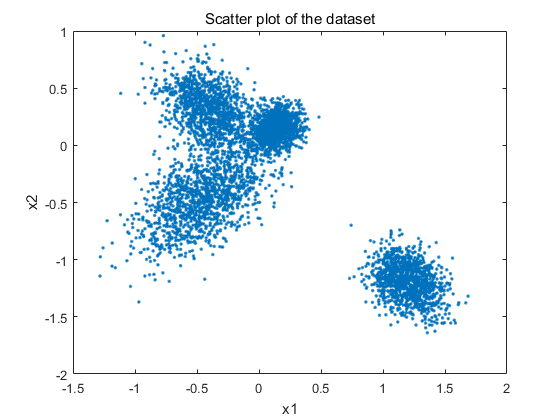
\includegraphics[width=10cm]{0}
  \caption{Scatter plot of the dataset}\label{0} 
\end{figure}

\subsection{Solutions to Problem 1)}
The in-complete data log-likelihood during training is shown in Fig.\ref{1-1}.
\begin{figure}
  \centering
  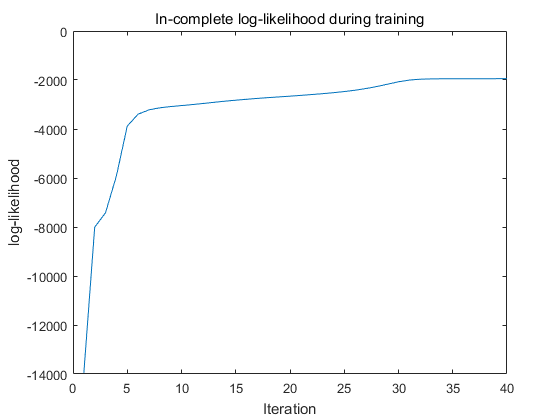
\includegraphics[width=10cm]{1-1}
  \caption{Plot of the in-complete log-likelihood $\ln p(X|\pi,\mu,\Sigma)$}\label{1-1} 
\end{figure}
Note that the training converges after 35 iterations.

\subsection{Solutions to Problem 2)}
The learned parameters are:\\
$\pi = (0.2300,0.2287,0.2731,0.2682)^T$ \\
$\mu_1=  \left(
  \begin{array}{c}
          -0.5231 \\
          0.1750
 \end{array}
 \right)$,
$\mu_2=  \left(
  \begin{array}{c}
         -0.0511 \\
          0.2182
 \end{array}
 \right)$, 
$\mu_3=  \left(
  \begin{array}{c}
          -0.3396 \\
          -0.3706
 \end{array}
 \right)$,
$\mu_4=  \left(
  \begin{array}{c}
          1.2035 \\
          -1.1969
 \end{array}
 \right)$ \\
$\Sigma_1= \left(
  \begin{array}{cc}
          0.0203 & 0.0088\\
          0.0088 & 0.1418
  \end{array}
  \right)$,
$\Sigma_2= \left(
  \begin{array}{cc}
          0.0813 & -0.0251\\
          -0.0251 & 0.0192
  \end{array}
  \right)$,\\
$\Sigma_3= \left(
  \begin{array}{cc}
          0.1011 & 0.0773\\
          0.0773 & 0.1003
  \end{array}
  \right)$,
$\Sigma_4= \left(
  \begin{array}{cc}
          0.0226 & -0.0076\\
          -0.0076 & 0.0236
  \end{array}
  \right)$

\subsection{Solutions to Problem 3)}
The scatter plot of $\gamma(z^{n})$ after training converges is depicted in Fig.\ref{1-2}.
\begin{figure}
  \centering
  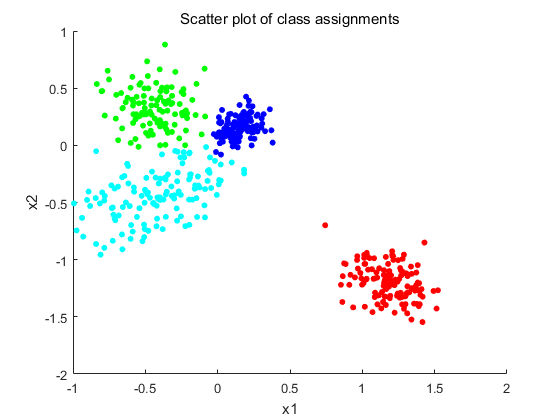
\includegraphics[width=10cm]{1-2}
  \caption{The scatter plot of $\gamma(z^{n})$ after training converges}\label{1-2} 
\end{figure}

\subsection{Solutions to Problem 4)}
If we initialize $\mu, \Sigma, \pi$ by other values, then the corresponding results are displayed in Fig.\ref{problem4}.

\begin{figure}
\centering
\begin{tabular}{cc}
\subf{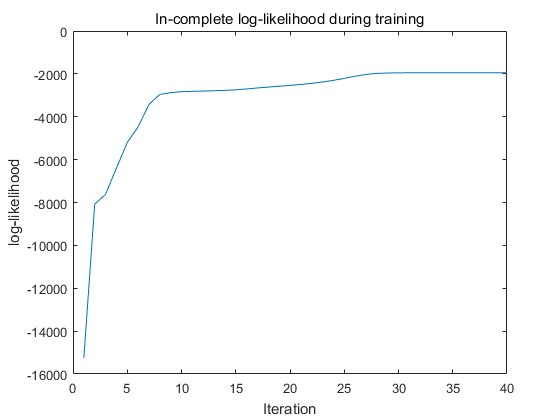
\includegraphics[width=60mm]{4-1}}
		{} % Can put caption for this subfigure here
&
\subf{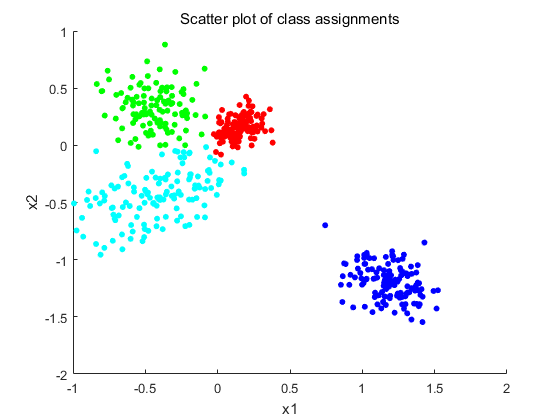
\includegraphics[width=60mm]{4-2}}
		{}
\\
\subf{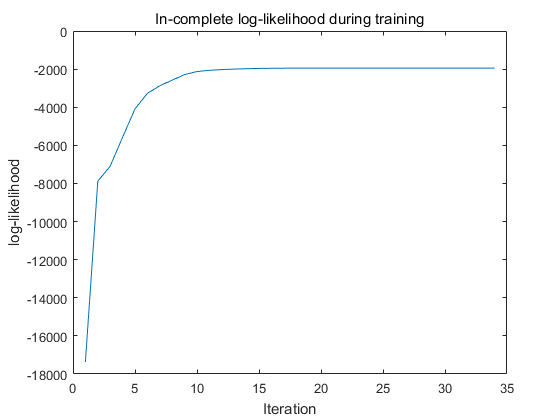
\includegraphics[width=60mm]{5-1}}
		{}
&
\subf{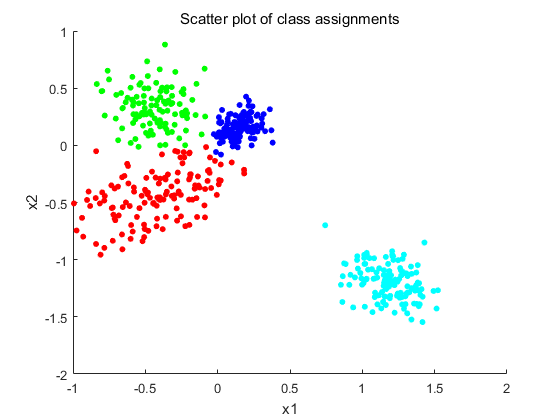
\includegraphics[width=60mm]{5-2}}
		{}
\\
\end{tabular}
\caption{log-likelihood and class assignments for two experiments}
\label{problem4}
\end{figure}
Note that under two experiment settings, the training process converges at different speed, but the convergence seems the same.

Although it seems no obvious difference in the figures above, we can observe the variation through the values of $\mu$. Here we show the values of $\mu$ from two experiments.
\begin{itemize}
	\item Experiment 1 \\
	$\mu_1=  \left(
  \begin{array}{c}
          -0.5231 \\
          0.1750
 \end{array}
 \right)$,
$\mu_2=  \left(
  \begin{array}{c}
         -0.0511 \\
          0.2182
 \end{array}
 \right)$, 
$\mu_3=  \left(
  \begin{array}{c}
          -0.3396 \\
          -0.3706
 \end{array}
 \right)$,
$\mu_4=  \left(
  \begin{array}{c}
          1.2035 \\
          -1.1969
 \end{array}
 \right)$ 
 	\item Experiment 2\\
 	$\mu_1=  \left(
  \begin{array}{c}
          -0.4423 \\
          0.4523
 \end{array}
 \right)$,
$\mu_2=  \left(
  \begin{array}{c}
         -0.4658 \\
          0.3215
 \end{array}
 \right)$, 
$\mu_3=  \left(
  \begin{array}{c}
          0.1444 \\
          0.1461
 \end{array}
 \right)$,
$\mu_4=  \left(
  \begin{array}{c}
          1.2035 \\
          -1.1969
 \end{array}
 \right)$ 
\end{itemize}

Note that $\mu_4$ is the same in two experiments as group 4 departs clearly from other groups, which is consistent with the figures above. However, $\mu_1, \mu_2, \mu_3$ are quite different as group $1 \sim 3$ mixes together and thus hard to classify.


\section{Conclusions}
EM algorithm can be used to derive the solution for Gaussian Mixture Models. Furthermore, the algorithm is quite sensitive to the initialization of the parameters.

\end{spacing}
\end{document}